\subsection{Análisis exploratorio de datos}
Se realizó un análisis exploratorio de los datos, el cuál permitió identificar valores de estadística descriptiva de los precios de cada uno de los productos. Para este análisis solamente se tomó en cuenta los precios de los últimos 6 años.

Este proceso adicionalmente implementó un proceso de limpieza de datos, donde se logró estandarizar los diferentes formatos de fecha presentes, así como extraer información como año, mes y trimestre del año.

Teniendo los datos preparados se procedió a obtener gráficas de la distribución del precio de cada producto a lo largo de los diferentes años analizados, así como gráficas que permiten realizar un análisis del precio de los productos en cada trimestre y cómo fue su comportamiento a lo largo de todos los años analizados.


\subsection{Funciones de aptitud}
Partiendo del modelo básico de optimización de precio, se procedió a generar datos sintéticos para el inventario de cada uno de los productos a lo largo del periodo analizado. Este proceso de generación de datos sintéticos se realizó con las siguientes reglas:

\begin{itemize}
	\item Valor máximo: $10,000$ toneladas.
	\item Valor mínimo: $2,000$ toneladas.
	\item Valor promedio: $5,000$ toneladas.
	\item Desviación estándar:
	\begin{itemize}
		\item Lactosa: $2,000$ toneladas.
		\item Suero: $1,500$ toneladas.
	\end{itemize}
\end{itemize}

Teniendo los datos sintéticos de inventario, se insertaron de forma aleatoria a nuestro conjunto de datos para simular la demanda del producto ante cada precio, donde se tomó la asunción de una venta completa, es decir, la demanda del producto fue la misma que le inventario.

Teniendo las consideraciones anteriores, se procedió a obtener un modelo lineal que se ajuste a la variación de la demanda según el precio. Estos modelos lineales siguen la forma de la función de demanda (Ecuación \ref{eq:demand}).

Una vez estimada la función de demanda para cada producto de interés, se procedió a implementar la función de ganancia (Ecuación \ref{eq:revenue}) con una ligera variación. Considerando que se tienen 2 tipos de cliente (un cliente estándar que compra poco producto y suele tener un precio estándar; un cliente premium que compra grandes cantidades de producto y suele tener un descuento al precio estándar), se procedió a modificar la función de ganancia para que esta considere el precio mas un 10\%, al realizar esta modificación incrementamos el precio para el cliente estándar, permitiendo también que al cliente premium le apliquemos un descuento y no perdamos ganancias. Tomando esas consideraciones finales, el modelo básico de optimización de precio se estableció como la Ecuación\ref{eq:price2}

\begin{equation}\label{eq:price2}
	R(p)= (p+0.10*p)(a-b(p+0.10*p))
\end{equation}


\subsection{Algoritmo genético}
Para esta práctica se desarrolló un algoritmo genético que se apega al proceso mostrado en la Figura \ref{fig:AG}.

\begin{figure}[htbp]
	\centering
	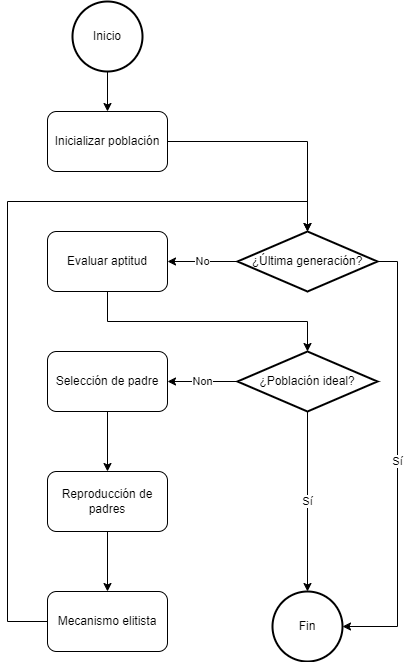
\includegraphics[width=0.35\textwidth]{algoritmo_genetico_proceso}
	\caption{Diagrama de flujo del algoritmo genético implementado.}
	\label{fig:AG}
\end{figure}

Para llevar a cabo dicho proceso, se optó por utilizar el lenguaje de programación Python, donde se diseñaron métodos genéricos para realizar los procesos de generación de población, evaluación de aptitud, selección de individuos, reproducción de individuos, mutación y mecanismos elitistas.


\subsection{Implementación de algoritmo en Python}
\subsubsection{Inicializador de población}
\begin{minted}
[
baselinestretch=1.2,
fontsize=\scriptsize,
linenos
]
{python}
def init_binary_population(n: int = 10, genes: int = 10):
    min = 0
    max = 2**genes
    population = np.random.randint(min, max, n)
    population = [int_to_bin_array(individue, genes) for individue in population]
    population = np.array(population)
    
    return population
\end{minted}


\subsubsection{Evaluación de individuos}
\begin{minted}
[
baselinestretch=1.2,
fontsize=\scriptsize,
linenos
]
{python}
def evaluate_binary_aptitude(individue: np.ndarray, domain: tuple, aptitude_function: callable):
    bits = individue.shape[0]
    min = 0
    max = 2**bits - 1
    decoded_individue = bin_array_to_int(individue)
    decoded_individue = (decoded_individue - min) / (max - min)
    decoded_individue = (domain[1] - domain[0]) * decoded_individue + domain[0]
    aptitude = aptitude_function(decoded_individue)
    
    return aptitude


def evaluate_population(population: np.ndarray, domain: tuple, aptitude_function: callable, desc: bool = True):
    aptitudes = np.vstack([evaluate_binary_aptitude(individue, domain, aptitude_function) for individue in population])

    direction = -1 if desc else 1
    sorted_indexes = aptitudes[:, -1].argsort()[::direction]
    sorted_population = population[sorted_indexes]
    sorted_aptitudes = aptitudes[sorted_indexes]
    avg_aptitude = np.mean(sorted_aptitudes)
    max_aptitude = np.max(sorted_aptitudes)

    return sorted_population, sorted_aptitudes, avg_aptitude, max_aptitude
\end{minted}


\subsubsection{Selección de parejas}
\begin{minted}
[
baselinestretch=1.2,
fontsize=\scriptsize,
linenos
]
{python}
def polygamous_random_selection(population: np.ndarray):
    n_couples = population.shape[0]//2
    couples = np.random.choice(population.shape[0], (n_couples, 2), replace=True)

    return couples
\end{minted}


\subsubsection{Reproducción de individuos}
\begin{minted}
[
baselinestretch=1.2,
fontsize=\scriptsize,
linenos
]
{python}
def two_point_crossover(population: np.ndarray, parents: np.ndarray):
    childrens = np.empty_like(population)
    for idx, couple in enumerate(parents):
        crossover_point = population.shape[1]//3
        childrens[idx*2, :crossover_point] = population[couple[0], :crossover_point]
        childrens[idx*2, crossover_point:2*crossover_point] = population[couple[1], crossover_point:2*crossover_point]
        childrens[idx*2, 2*crossover_point:] = population[couple[0], 2*crossover_point:]
        childrens[idx*2+1, :crossover_point] = population[couple[1], :crossover_point]
        childrens[idx*2+1, crossover_point:2*crossover_point] = population[couple[0], crossover_point:2*crossover_point]
        childrens[idx*2+1, 2*crossover_point:] = population[couple[1], 2*crossover_point:]

    return childrens
\end{minted}


\subsubsection{Mutación}
\begin{minted}
[
baselinestretch=1.2,
fontsize=\scriptsize,
linenos
]
{python}
def inverse_mutation(individues: np.ndarray, mr: float = 0.02):
    total_individues = individues.shape[0]
    individue_len = individues.shape[1]
    to_mutate = np.random.choice(total_individues, int(total_individues*mr))

    for idx in to_mutate:
        idx_l, idx_r = sorted(np.random.choice(individue_len, 2))
        idx_r = idx_r if idx_r == 17 else idx_r + 1
        individues[idx][idx_l:idx_r] = individues[idx][idx_l:idx_r][::-1]

    return individues
\end{minted}


\subsubsection{Elitismo}
\begin{minted}
[
baselinestretch=1.2,
fontsize=\scriptsize,
linenos
]
{python}
def genetic_competence(population: np.ndarray, childrens: np.ndarray):
    all_population = np.vstack([population, childrens])
    sorted_population, _, _, _ = evaluate_population(all_population, (0, 5), revenue_lactose)
    return sorted_population[:population.shape[0]]
\end{minted}


\subsubsection{Algoritmo completo}
\begin{minted}
[
baselinestretch=1.2,
fontsize=\scriptsize,
linenos
]
{python}
lactose_population = init_binary_population(100, 2**4)
generations = 15
epsilon = 3000
last_avg_aptitude = float("inf")
max_stagnant_generations = 3
stagnant_generations = 0
delta = 30

avg_aptitudes_l = []
max_aptitudes_l = []
evolution_l = []

for _ in range(generations):
    lactose_population, _, avg_aptitude, max_aptitude = evaluate_population(lactose_population, (0, 5), revenue_lactose)
    avg_aptitudes_l.append(avg_aptitude)
    max_aptitudes_l.append(max_aptitude)
    evolution_l.append(lactose_population.copy())
    
    if abs(avg_aptitude - last_avg_aptitude) < delta:
        stagnant_generations += 1
        if stagnant_generations > max_stagnant_generations:
            break
    else:
        stagnant_generations = 0

    last_avg_aptitude = avg_aptitude
    parents = polygamous_random_selection(lactose_population)
    childrens = two_point_crossover(lactose_population, parents)
    childrens = inverse_mutation(childrens, 0.2)
    lactose_population = genetic_competence(lactose_population, childrens)
\end{minted}


\subsection{Pruebas realizadas}
Se implementó una solución en la cuál se utilizan poblaciones con codificación binaria, selección poligámica aleatoria, cruza de dos puntos, mutación por inversión y competencia genética.

Debido a que el objetivo es optimizar el precio de productos lacteos, se realizaron 2 ejecuciones del algoritmo, una para cada producto.

En cada ejecución del algoritmo se generaron gráficas que muestran el proceso de de evolución, en términos de aptitud y convergencia dentro del espacio de búsqueda.

El criterio de paro utilizado se estableció según los siguientes criterios:

\begin{itemize}
	\item Número de generaciones. Se estableció un límite de 15 generaciones para todos los algoritmos.
	\item Término por $\delta$. Se estableció un valor $\delta=30$ con un máximo de 3 generaciones.
\end{itemize}
